\documentclass{article}
\usepackage[utf8]{inputenc}
\usepackage[spanish]{babel}
\usepackage{graphicx, graphics, float, fancyhdr, titling}
\usepackage{listings, subcaption}
\usepackage[a4paper, total={6in, 9.5in}]{geometry}
\usepackage{hyperref}
\renewcommand{\footrulewidth}{0.4pt}
\title{

\includegraphics[width=1.75in]{imagenes/UGR-Logo.png} \\
\vspace*{1in}
\textbf{Práctica 1, Sesión 4} \\
Seguridad en Sistemas Operativos \\
\vspace*{0.5in}}
\author{Andrés Merlo Trujillo \\
\vspace*{0.5in} \\
E.T.S. de Ingenierías Informática y de Telecomunicación \\
\textbf{Universidad de Granada}} \date{\today}
%\date{}
\hypersetup{
    colorlinks=true,
    linkcolor=black,
}

\renewcommand\maketitlehooka{\null\mbox{}\vfill}
\renewcommand\maketitlehookd{\vfill\null}

\begin{document}
\begin{titlingpage}
    \maketitle
\end{titlingpage}

\tableofcontents

\newpage

\pagestyle{fancy}
\fancyhead[L]{Andrés Merlo Trujillo}
\fancyhead[R]{Seguridad en Sistemas Operativos}
%\addcontentsline{toc}{section}{Ejercicio 1}
%\section*{Ejercicio 1}
%\begin{figure}[H]
%    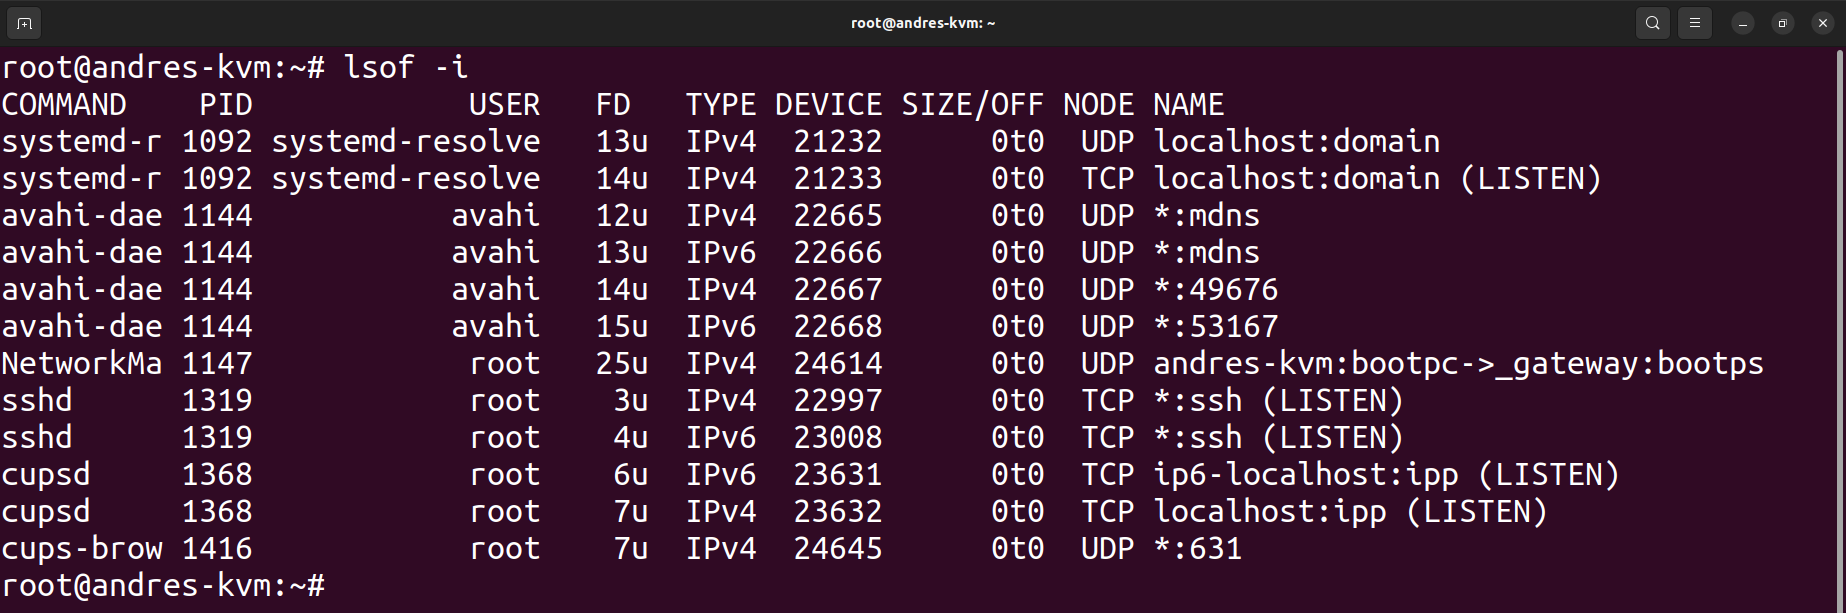
\includegraphics[width=\textwidth]{imagenes/lsofi.png}
%\end{figure}
\phantomsection
\addcontentsline{toc}{section}{Ejercicio 1}
\section*{Ejercicio 1}

\phantomsection
\addcontentsline{toc}{subsection}{Apartado A}
\subsection*{Apartado A}

\textbf{Enunciado: }``Utiliza la herramienta gpg para crear unas claves personales.''

\bigskip

Para crear las claves personales es necesario ejecutar la orden \verb|gpg --gen-key|. Ahora pedirá una serie de información que es necesario rellenar como el nombre o el correo.

%foto de nombre y apellidos.
\begin{figure}[H]
    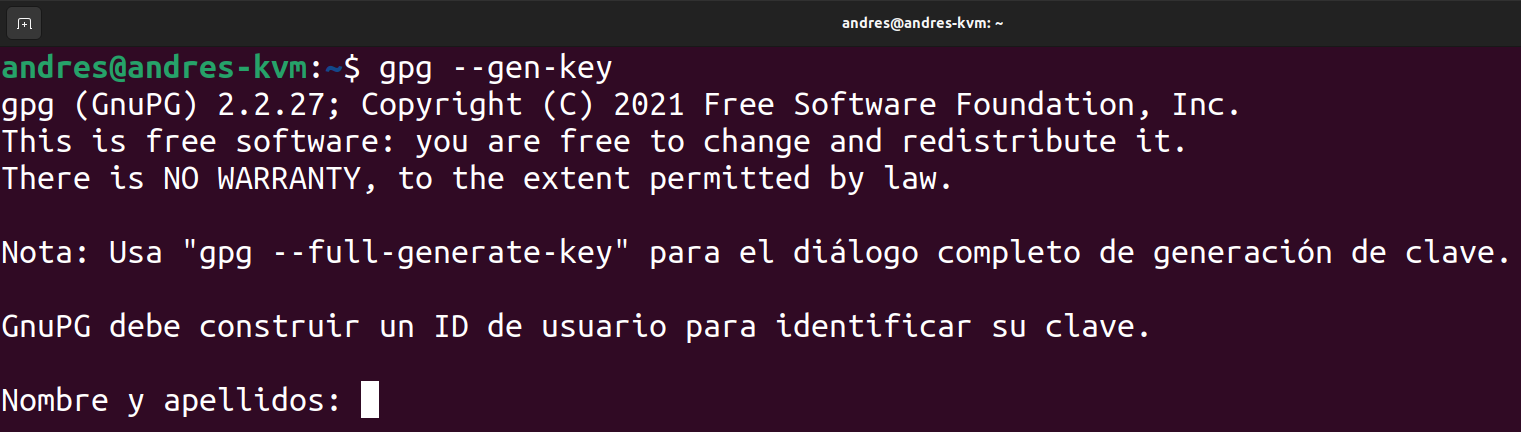
\includegraphics[width=\textwidth]{imagenes/Captura desde 2022-10-19 16-42-45.png}
    \caption{Generación de claves con la orden \texttt{gpg}.}
\end{figure}

A continuación aparece un sumario de los datos rellenados y al aceptarlos aparece un cuadro de texto para introducir la contraseña. Seguidamente, pide al usuario realizar diversas cosas para generar entropía y que la clave sea lo más aleatoria posible como mover el ratón, realizar actividad de red y de disco, etc.

\begin{figure}[H]
    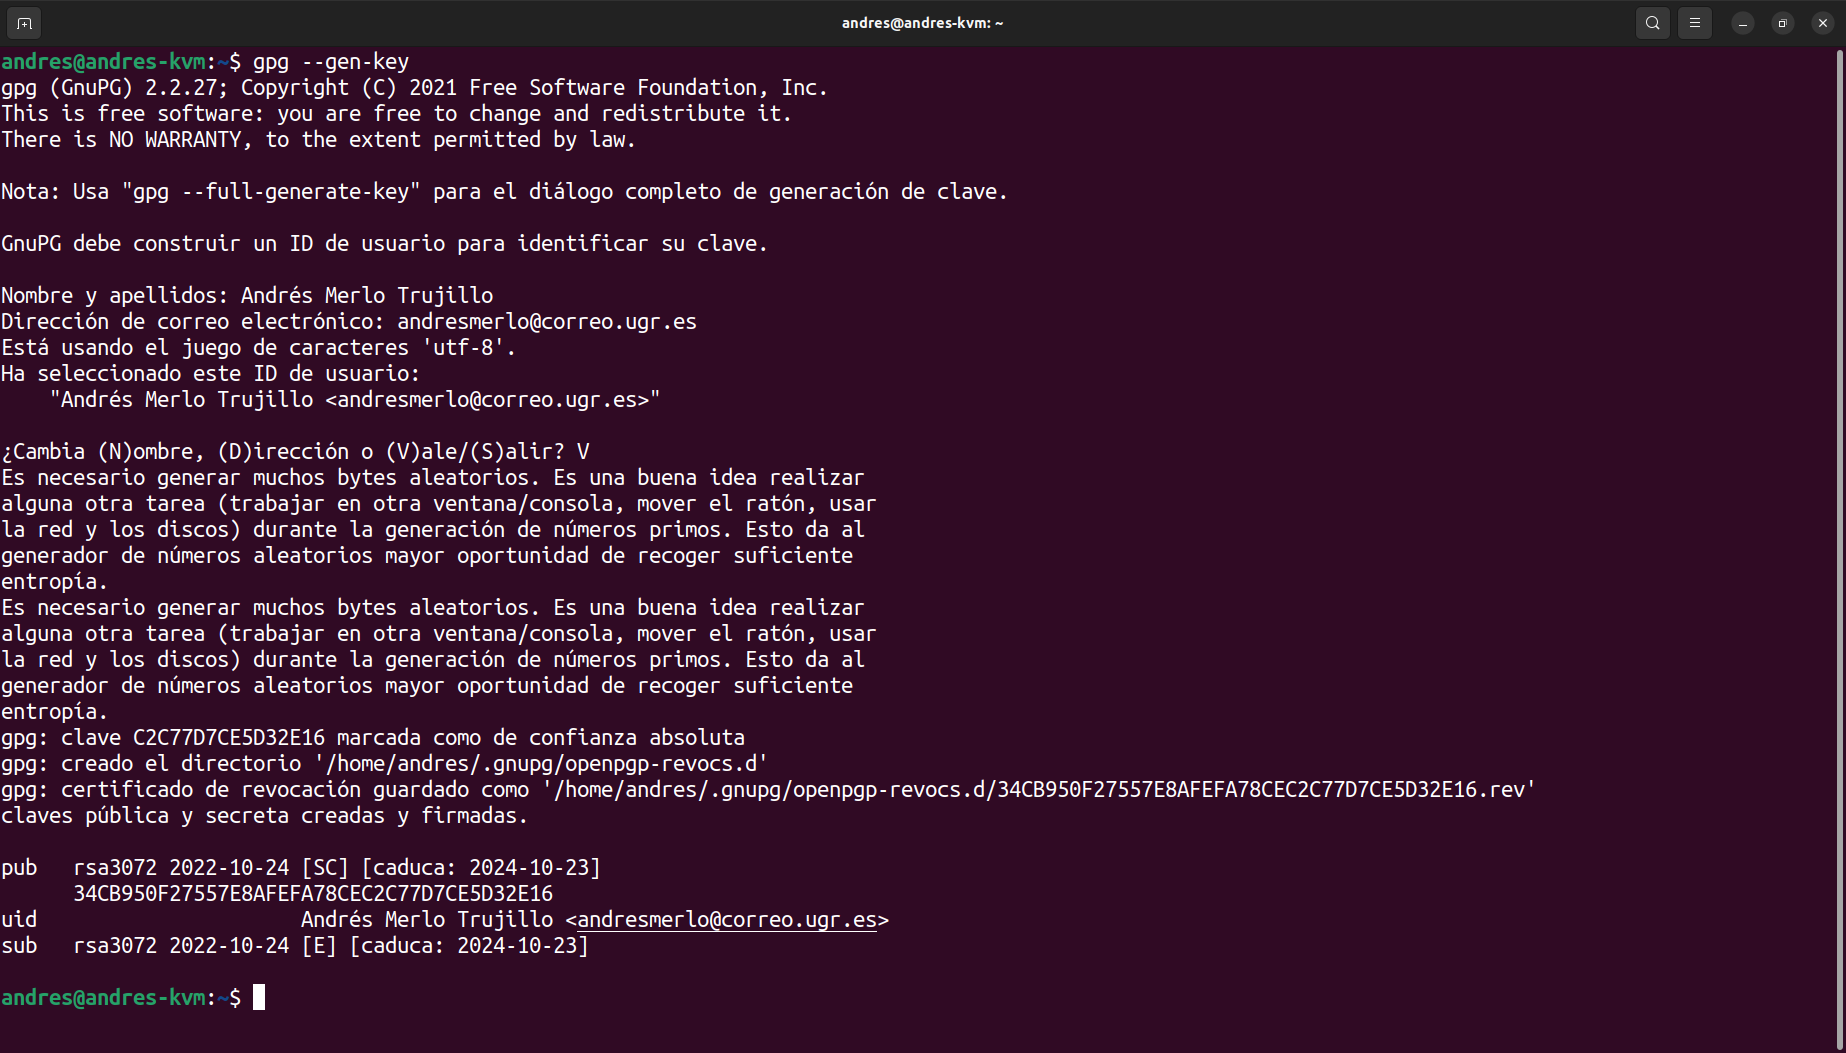
\includegraphics[width=\textwidth]{imagenes/Portatil/Captura desde 2022-10-24 11-46-02.png}
    \caption{Salida de la generación de claves.}
\end{figure}

\newpage

Y ahora para mostrar las claves públicas se utiliza el comando \verb|gpg --list-keys|:

%Captura desde 2022-10-19 16-55-18
\begin{figure}[H]
    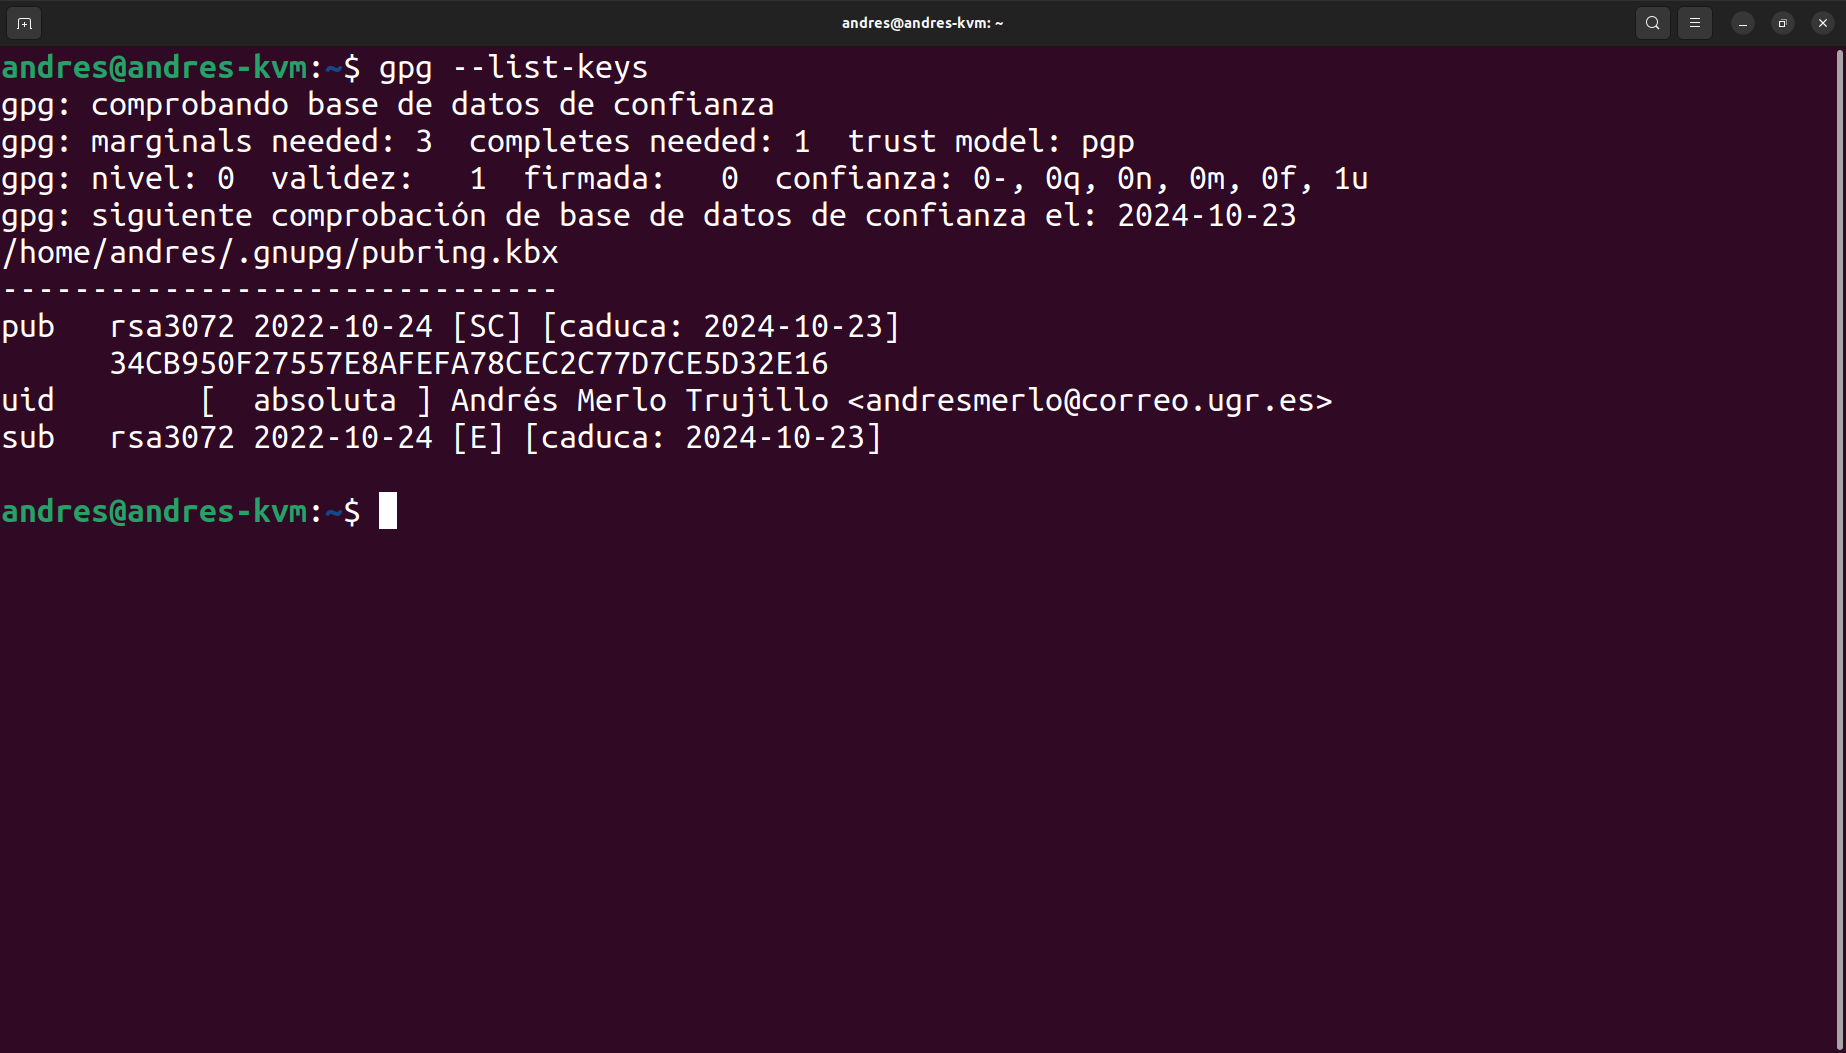
\includegraphics[width=\textwidth]{imagenes/Portatil/Captura desde 2022-10-24 11-46-16.png}
    \caption{Listado de claves públicas.}
\end{figure}

Y para mostrar las claves privadas se utiliza el comando \verb|gpg --list-secret-keys|:

%Captura desde 2022-10-19 16-55-26
\begin{figure}[H]
    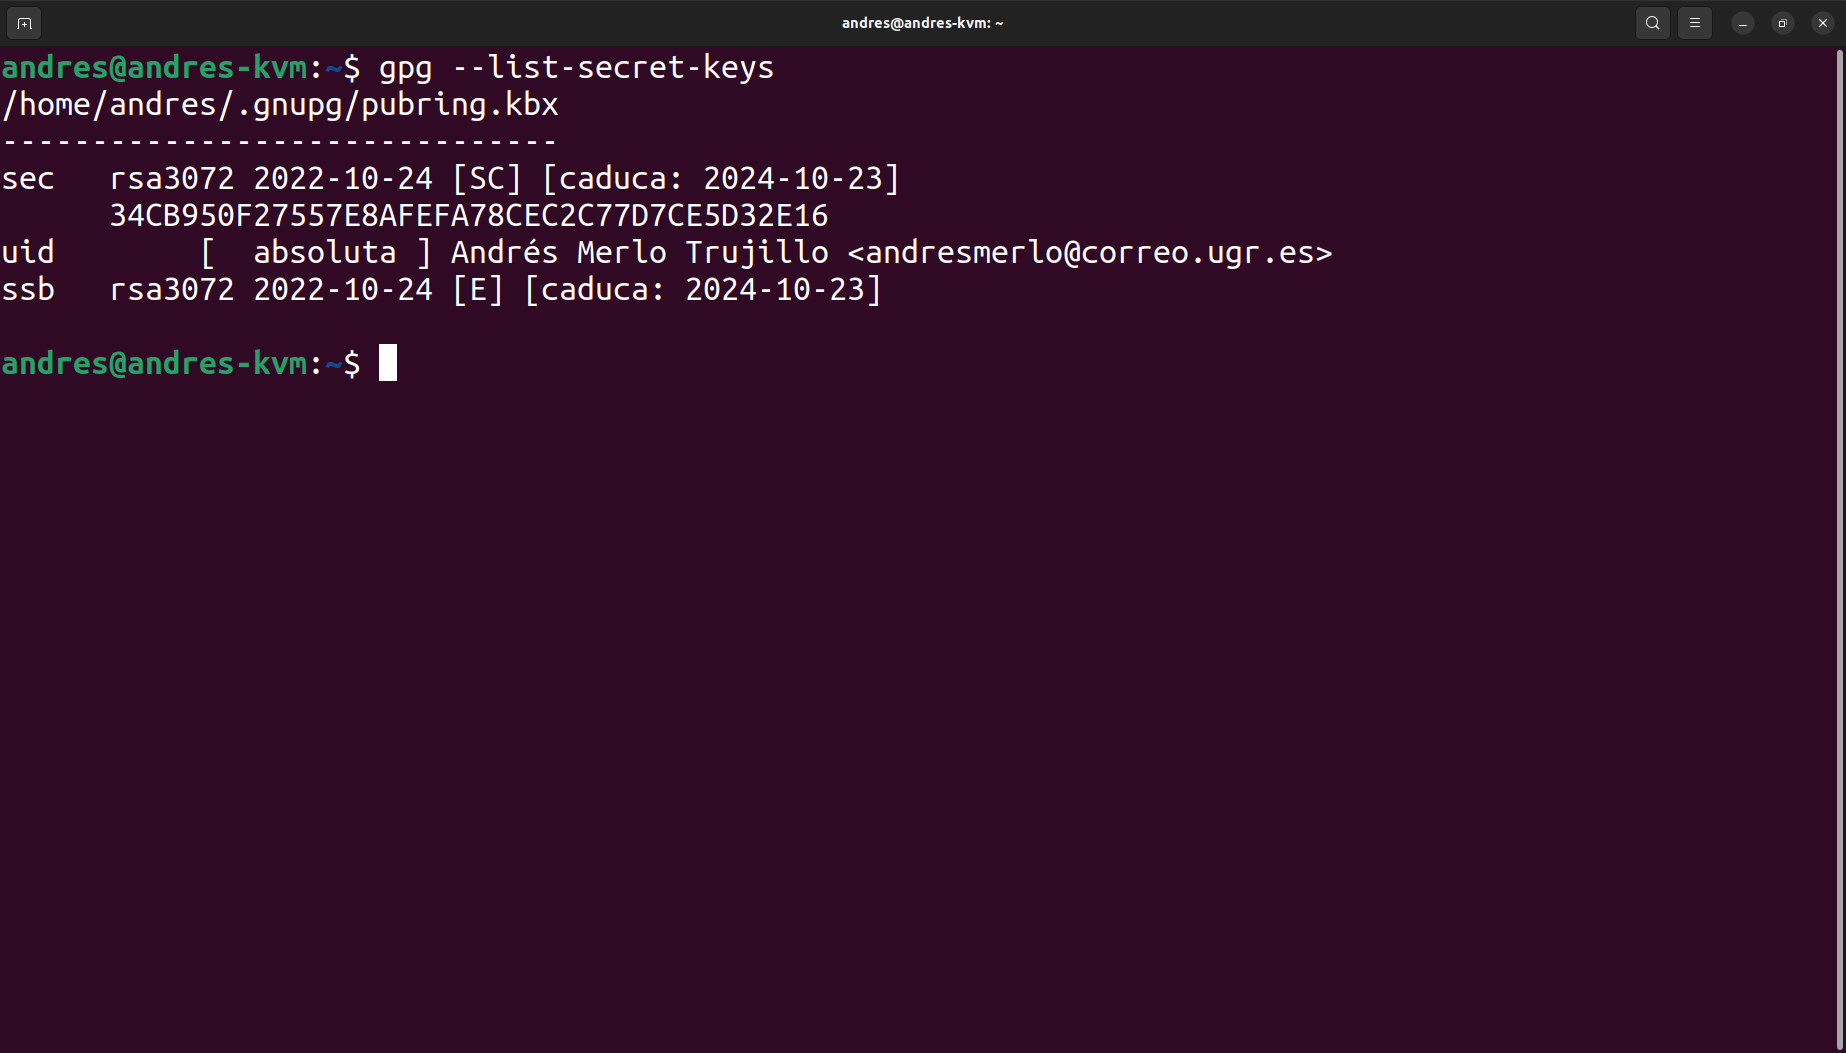
\includegraphics[width=\textwidth]{imagenes/Portatil/Captura desde 2022-10-24 11-46-25.png}
    \caption{Listado de claves privadas.}
\end{figure}

\phantomsection
\addcontentsline{toc}{subsection}{Apartado B}
\subsection*{Apartado B}

\textbf{Enunciado: }``Una vez creadas, utilízalas para cifrar y descifrar un archivo.''

\bigskip

Primero voy a crear un archivo de texto cualquiera como el siguiente:

%Captura desde 2022-10-19 16-57-15
\begin{figure}[H]
    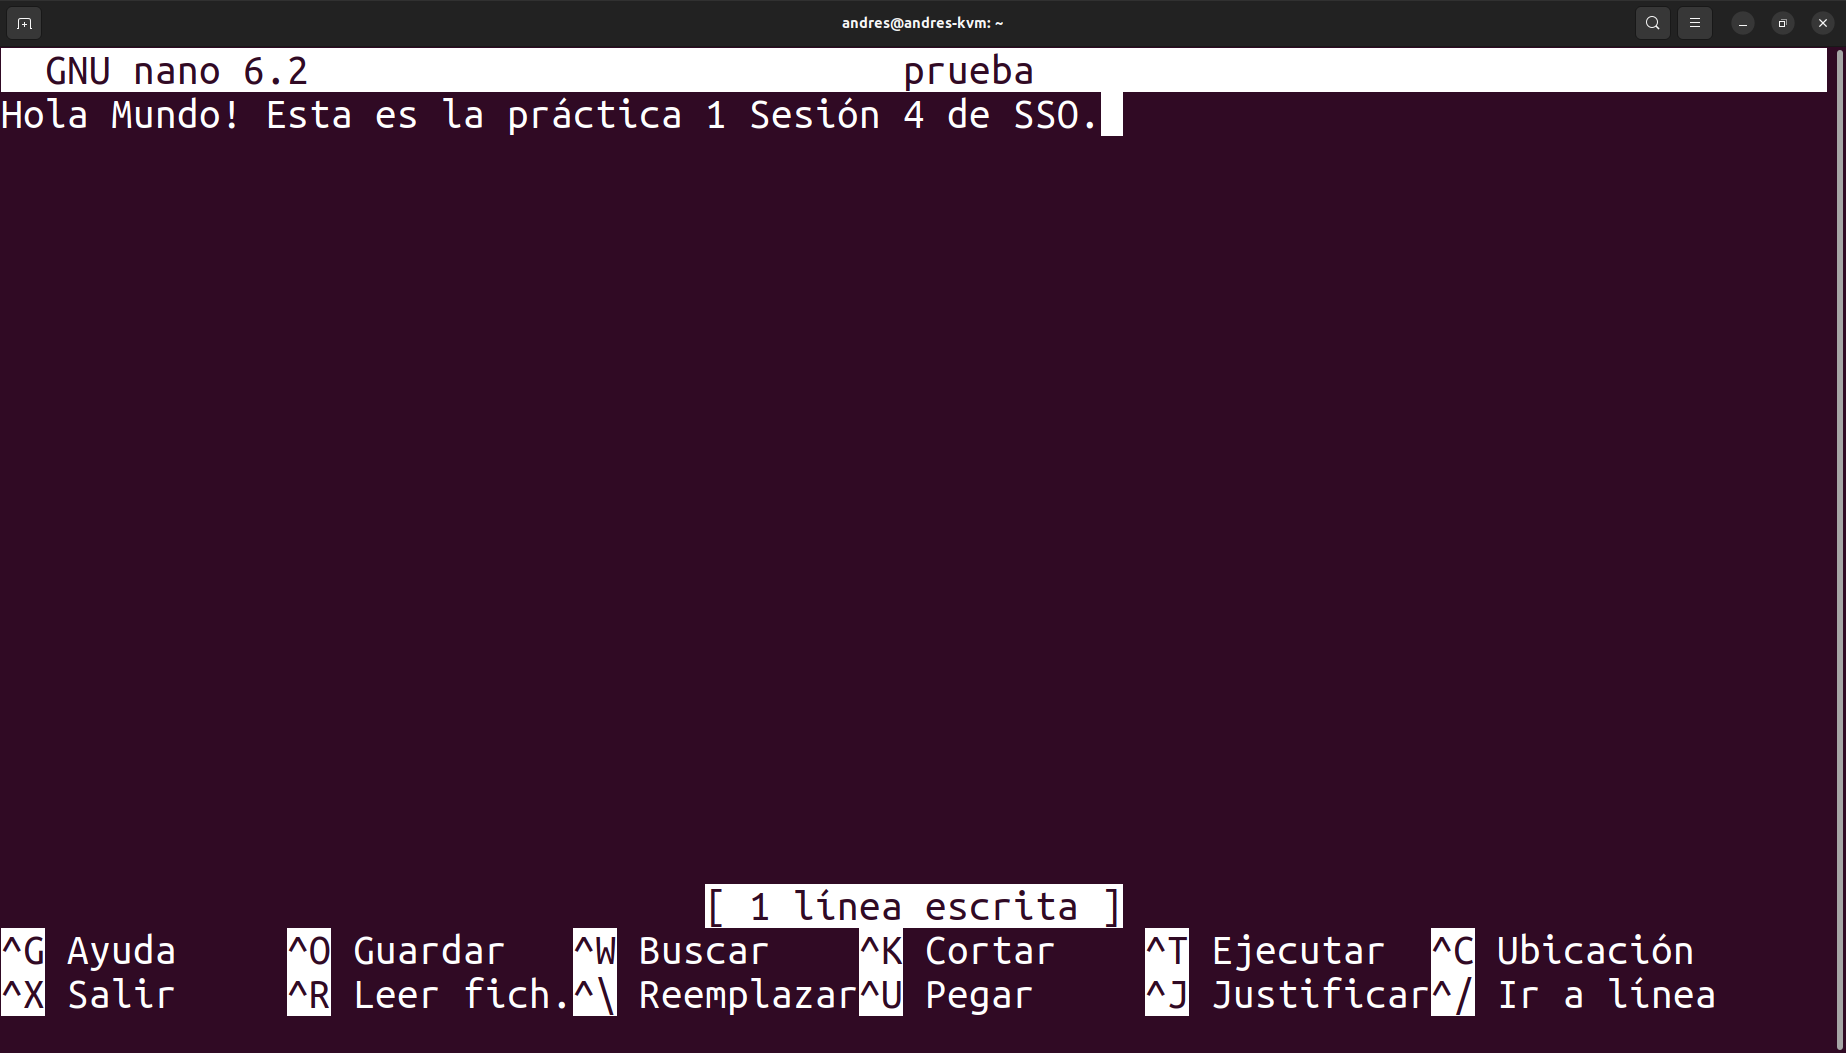
\includegraphics[width=\textwidth]{imagenes/Captura desde 2022-10-19 16-57-15.png}
    \caption{Mensaje a cifrar.}
\end{figure}

Para cifrar el archivo se utiliza la orden \verb|gpg --armor --recipient correo --encrypt file|. Para ello, en la parte de ``recipient'' es necesario poner el correo que se haya usado para crear las claves en el ejercicio anterior, o cualquier otro que se encuentre en un servidor como \verb|keyserver.ubuntu.com| o incluso importado localmente entre personas. Yo voy a realizar la primera de todas, encriptarlo con mi propia clave para mi correo.

\bigskip

Esto generará un fichero con la extensión ``.asc'' el cual, si se abre, contiene lo siguiente:

%Captura desde 2022-10-19 17-06-08
\begin{figure}[H]
    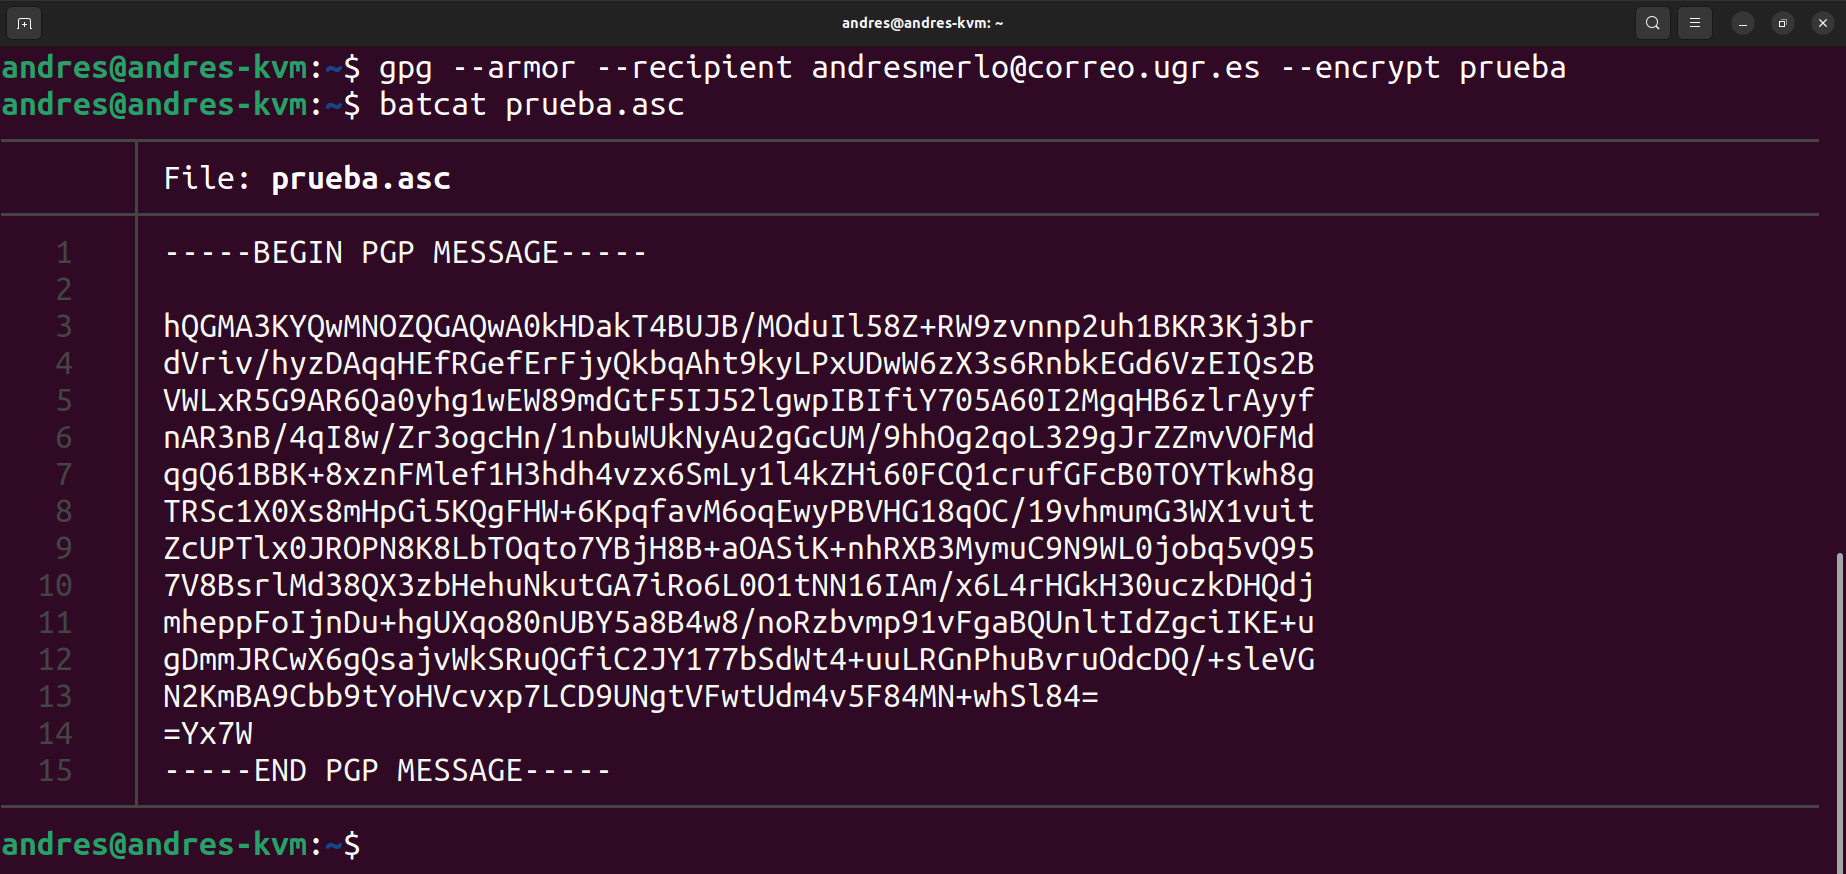
\includegraphics[width=\textwidth]{imagenes/Portatil/Captura desde 2022-10-27 18-34-40.png}
    \caption{Contenido del mensaje encriptado.}
\end{figure}


Por último, para descifrar el mensaje se utiliza la orden \verb|gpg --decrypt prueba.asc|, se pedirá la contraseña que se insertó al crear las claves.

%Captura desde 2022-10-19 17-07-30
\begin{figure}[H]
    \centering
    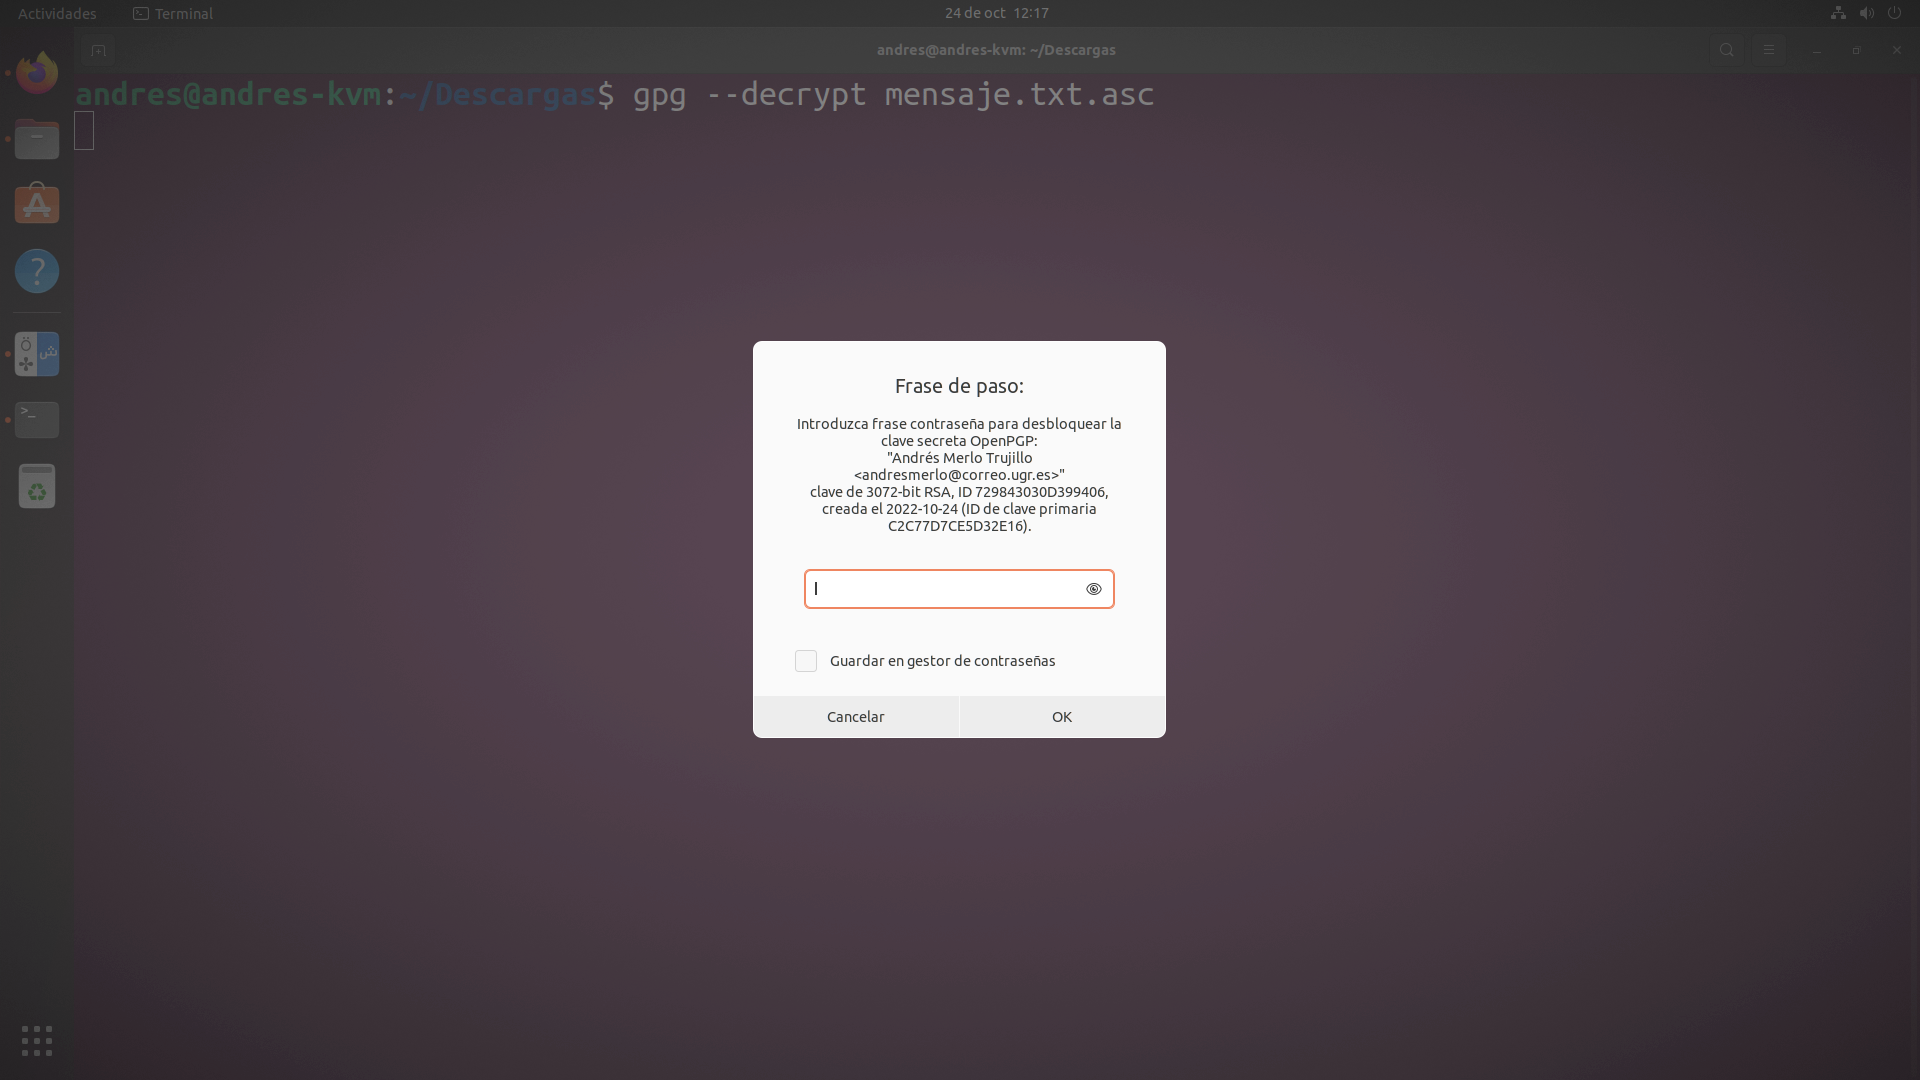
\includegraphics[width=0.6\textwidth]{imagenes/Portatil/Captura desde 2022-10-24 12-17-29.png}
    \caption{Contraseña de la clave para desencriptar el mensaje.}
\end{figure}

%Captura desde 2022-10-19 17-07-50
\begin{figure}[H]
    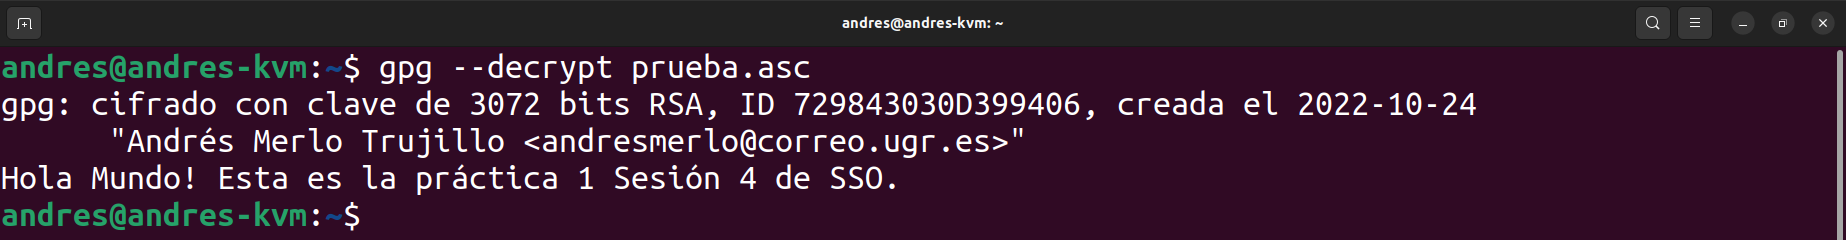
\includegraphics[width=\textwidth]{imagenes/Portatil/Captura desde 2022-10-27 18-35-01.png}
    \caption{Salida del mensaje desencriptado.}
\end{figure}


\phantomsection
\addcontentsline{toc}{subsection}{Apartado C}
\subsection*{Apartado C}

\textbf{Enunciado: }``Agrúpate con un compañero e intercambiar un archivo cifrado por cada uno que el otro debe descifrar.''

\bigskip

Me he juntado con Carlos Salas Eiroa (csalaseiroa@correo.ugr.es) para mandarnos archivos cifrados a cada uno.

Para que él pueda obtener mi clave pública, es necesario subirla a un servidor como \url{https://keyserver.ubuntu.com/}. Para ello, necesito obtener el ID de la clave pública mía en formato corto con la orden \verb|gpg --list-keys --keyid-format SHORT|.


\begin{figure}[H]
    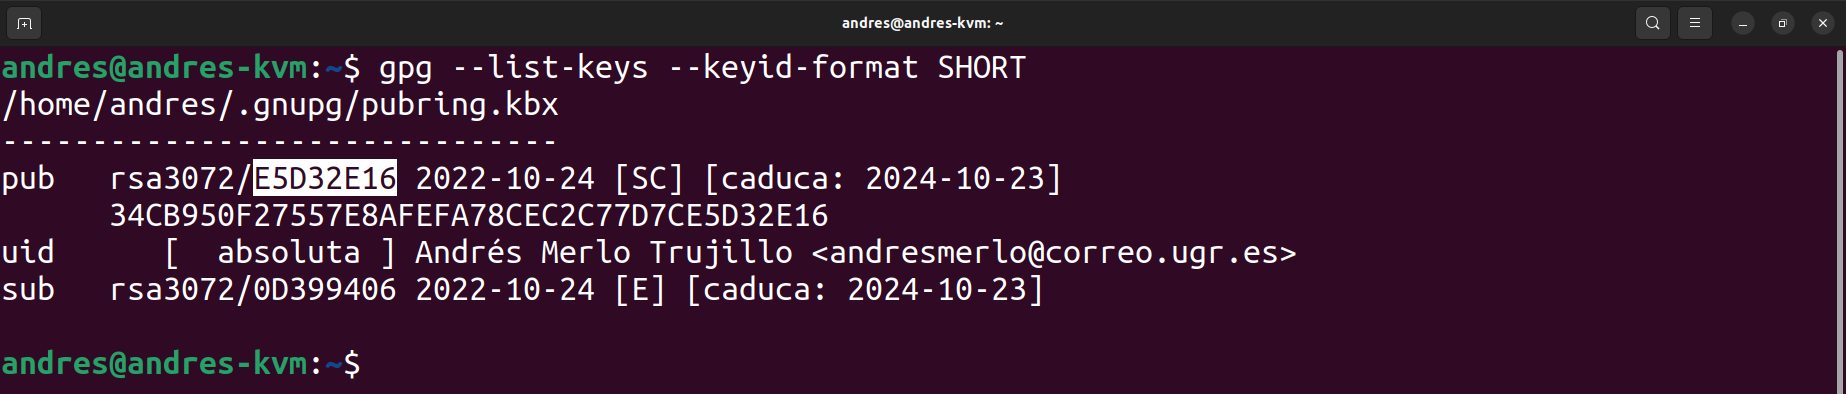
\includegraphics[width=\textwidth]{imagenes/Portatil/Captura desde 2022-10-24 11-54-58.png}
    \caption{El ID corto se encuentra en la tercera línea después de ``rsa3072/''.}
\end{figure}

Y una vez obtenido el ID en formato corto, con la orden:

\verb|gpg --send-keys --keyserver keyserver.ubuntu.com SHORT_ID| se envía al servidor. 

%Captura desde 2022-10-24 11-58-08
\begin{figure}[H]
    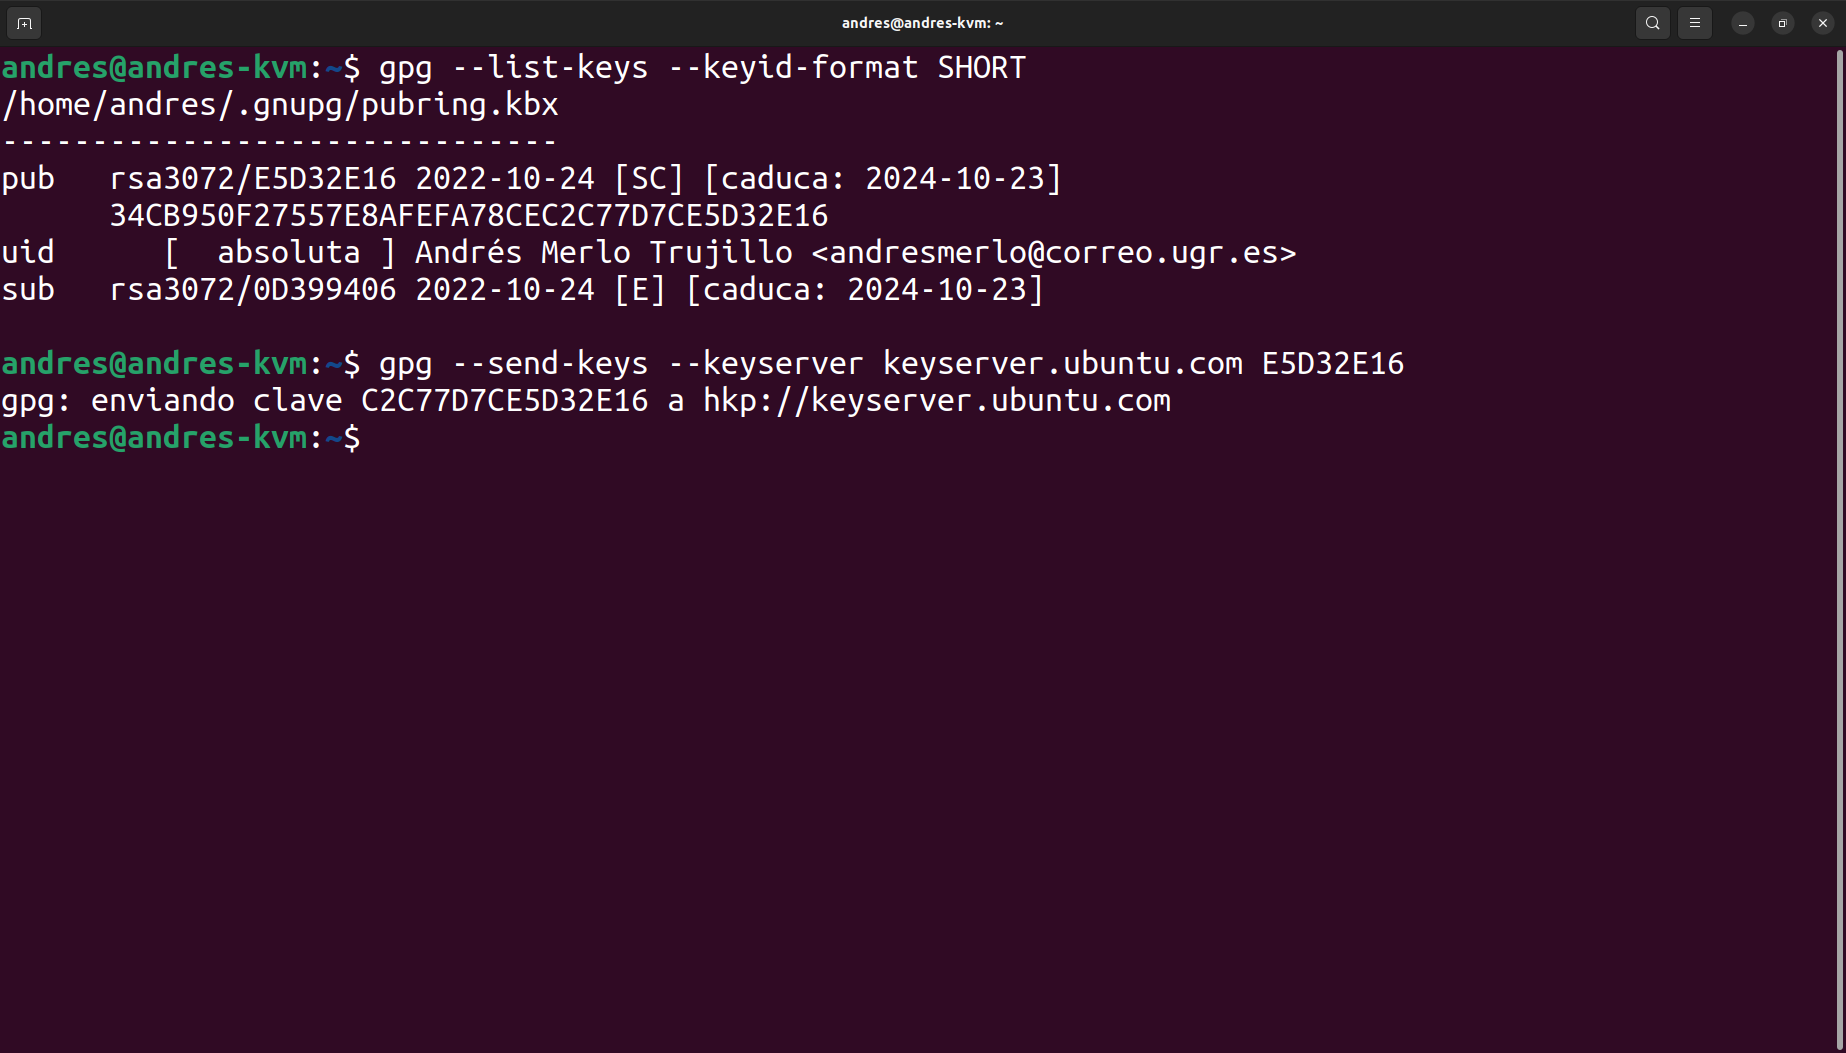
\includegraphics[width=\textwidth]{imagenes/Portatil/Captura desde 2022-10-24 11-58-08.png}
    \caption{Envío de clave pública al servidor de claves de Ubuntu.}
\end{figure}

Y si todo se ha realizado correctamente, al buscar mi clave pública en el servidor debería aparecer:


\begin{figure}[H]
    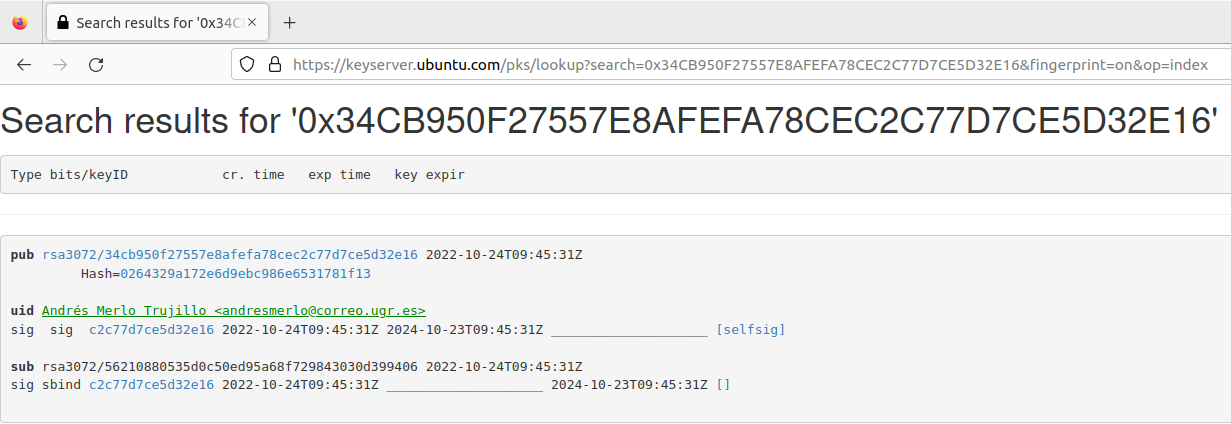
\includegraphics[width=\textwidth]{imagenes/Portatil/Captura desde 2022-10-24 12-01-53.png}
    \caption{Aparece correctamente en la página.}
\end{figure}

\newpage

Y mi compañero también ha subido la suya:

\begin{figure}[H]
    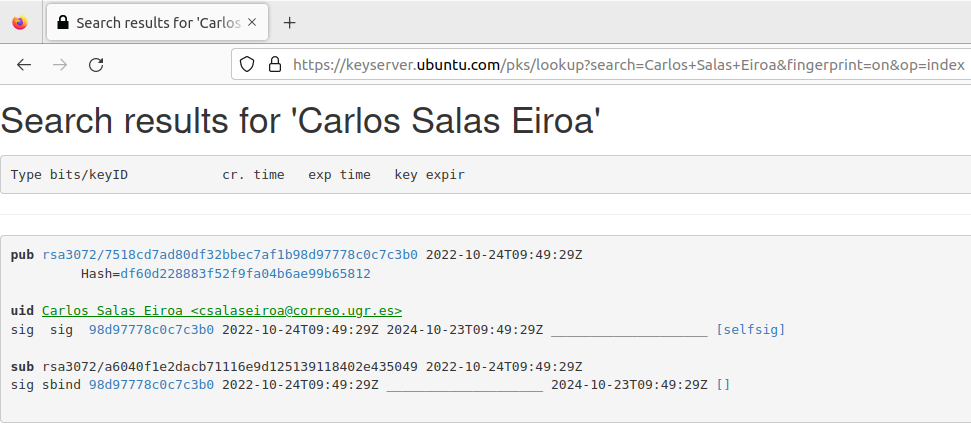
\includegraphics[width=\textwidth]{imagenes/Portatil/Captura desde 2022-10-24 12-05-30.png}
    \caption{Aparece correctamente la clave pública de mi compañero.}
\end{figure}


A continuación, he creado el siguiente archivo para mi compañero:

\begin{figure}[H]
    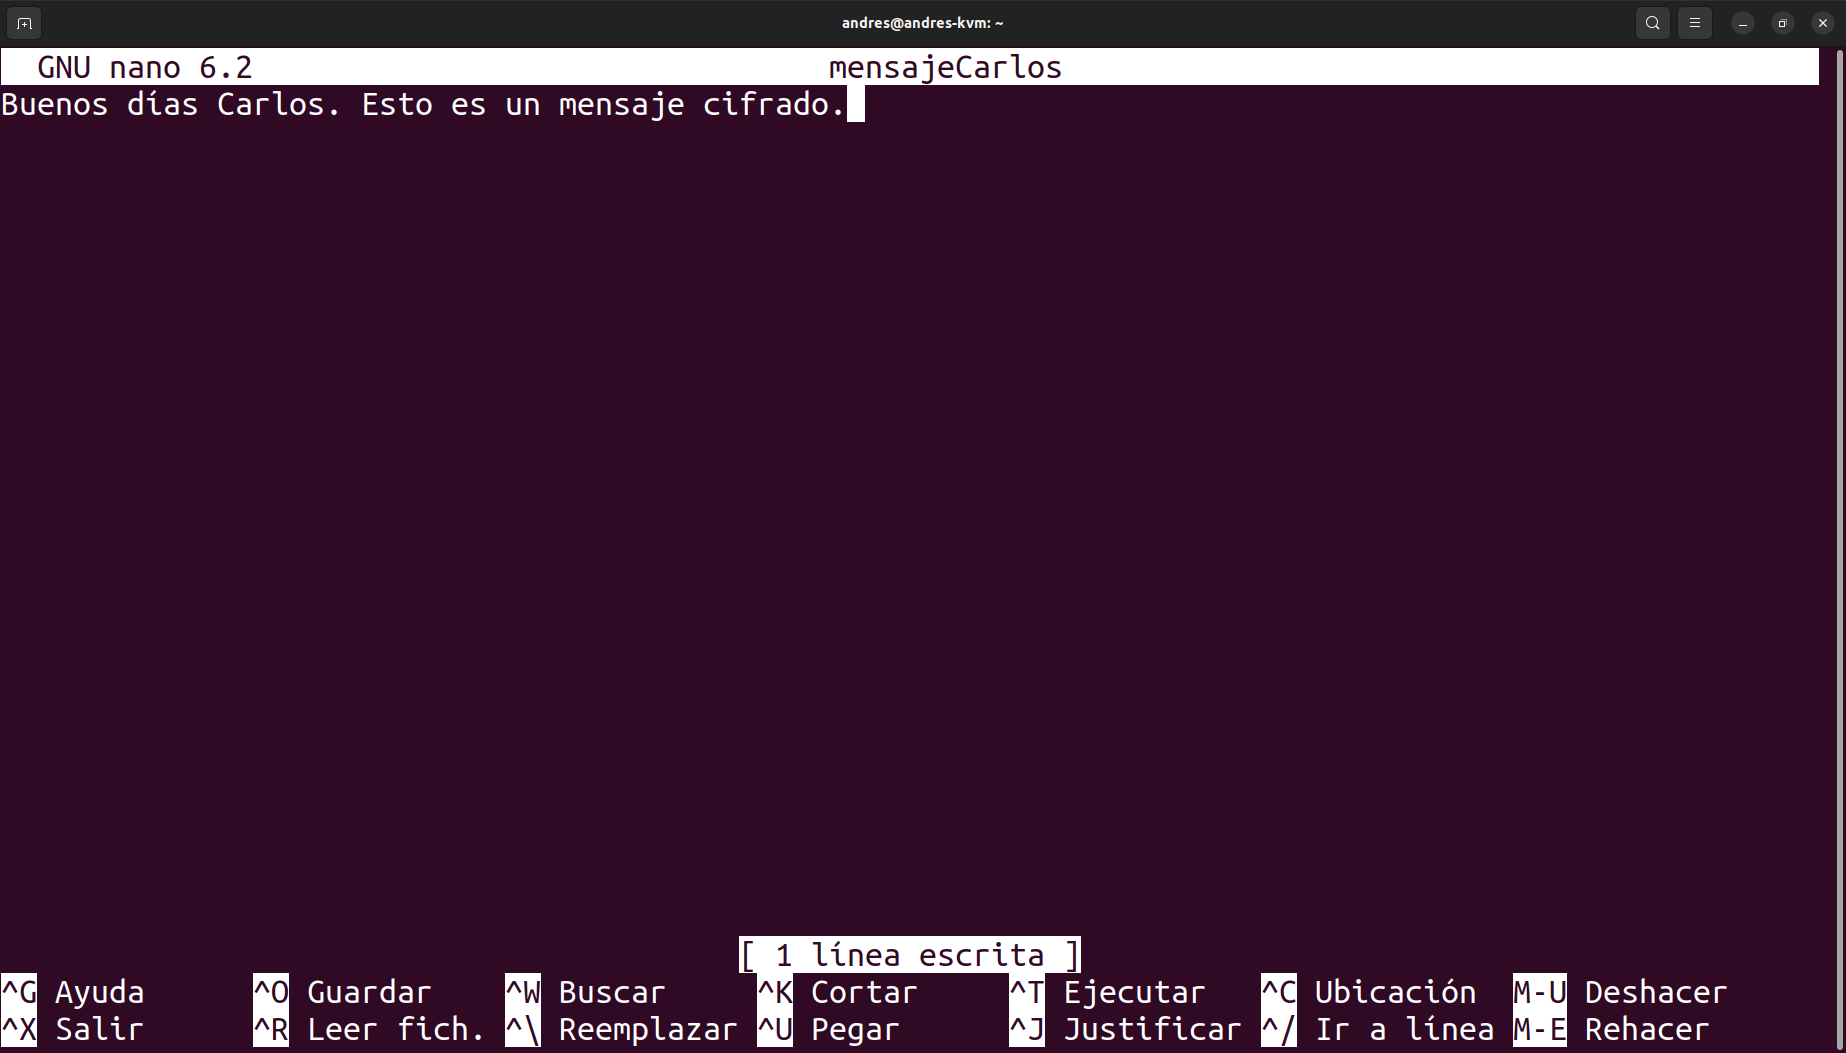
\includegraphics[width=\textwidth]{imagenes/Portatil/Captura desde 2022-10-24 12-02-33.png}
    \caption{Mensaje que voy a cifrar para enviárselo a mi compañero.}
\end{figure}

Y necesito su clave pública del servidor para poder encriptarlo y que solo él pueda leerlo, para ello, con el comando \verb|gpg --keyserver keyserver.ubuntu.com --recv-keys SHORT_ID| obtengo su clave pública:

\begin{figure}[H]
    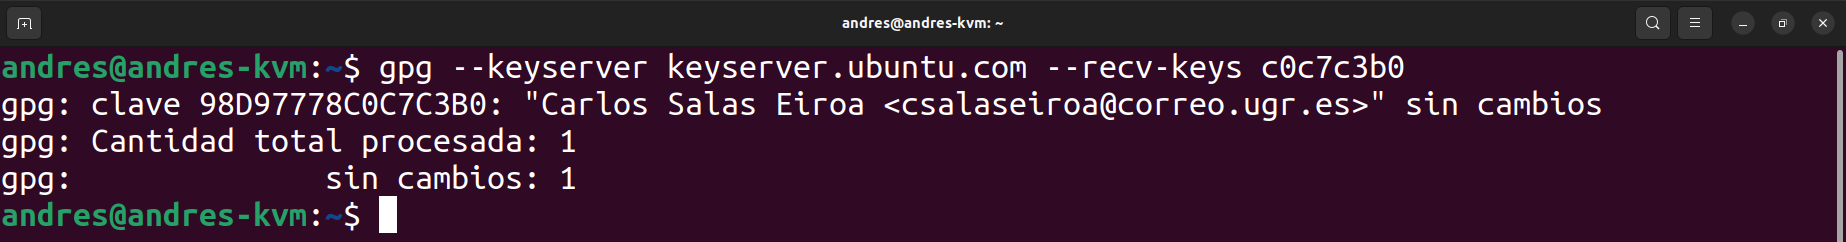
\includegraphics[width=\textwidth]{imagenes/Portatil/Captura desde 2022-10-24 12-11-03.png}
    \caption{Primero hace falta recibir la clave pública de Carlos.}
\end{figure}

Y con la orden \verb|gpg --armor --recipient correo --encrypt file| se encripta y se puede mandar el archivo con extensión ``.asc'' sin problema por correo electrónico.

\begin{figure}[H]
    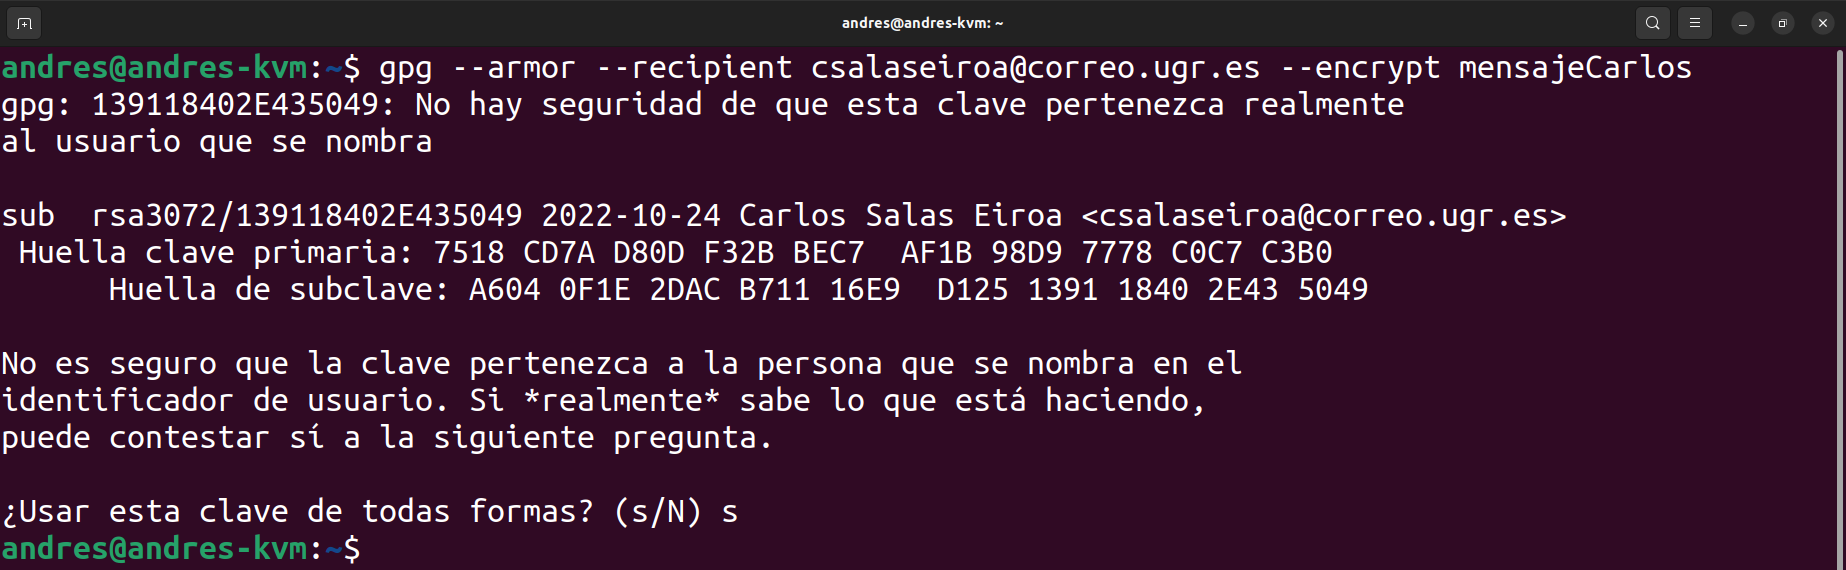
\includegraphics[width=\textwidth]{imagenes/Portatil/Captura desde 2022-10-24 12-11-31.png}
    \caption{Encriptación de mi mensaje con la clave pública de Carlos.}
\end{figure}


Ahora, me descargo el archivo que mi compañero me ha enviado por correo electrónico:

\begin{figure}[H]
    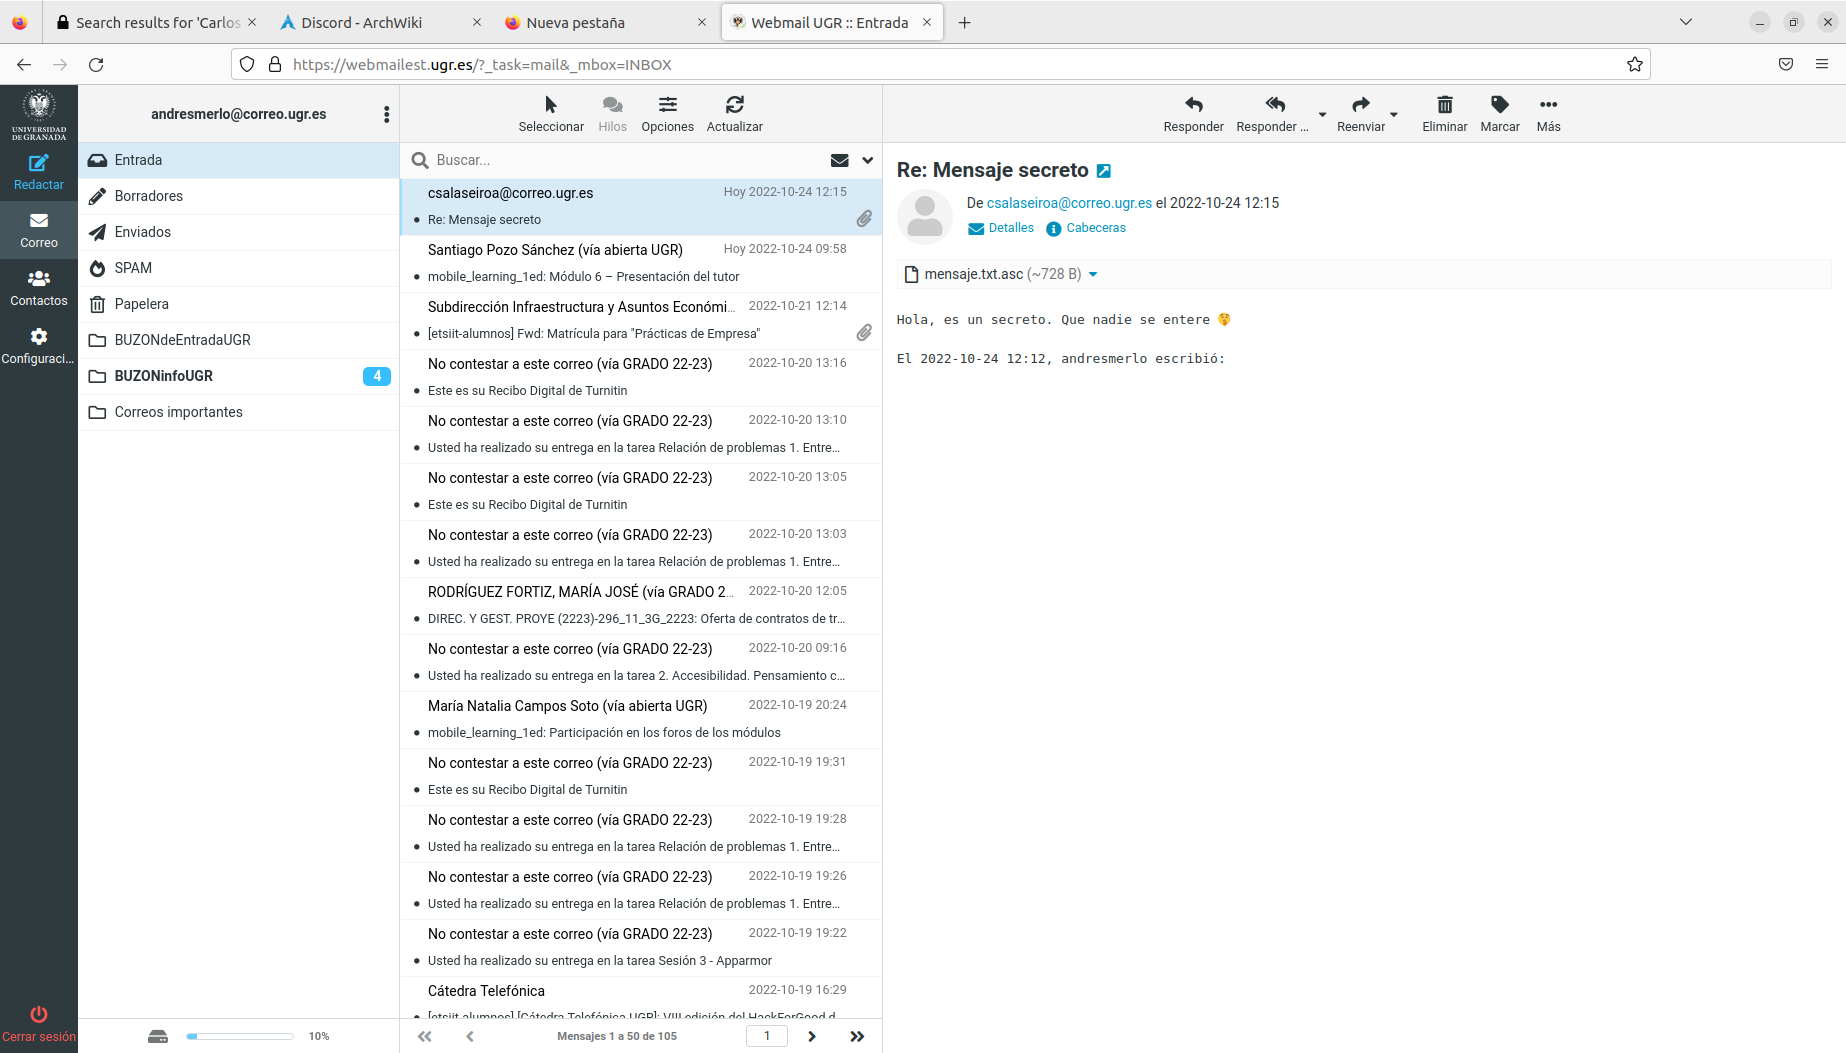
\includegraphics[width=0.9\textwidth]{imagenes/Portatil/Captura desde 2022-10-24 12-16-48.png}
    \caption{Mensaje recibido de Carlos.}
\end{figure}

A continuación, usando la orden \verb|gpg --decrypt file| se puede abrir el archivo que mi compañero me ha enviado.

\begin{figure}[H]
    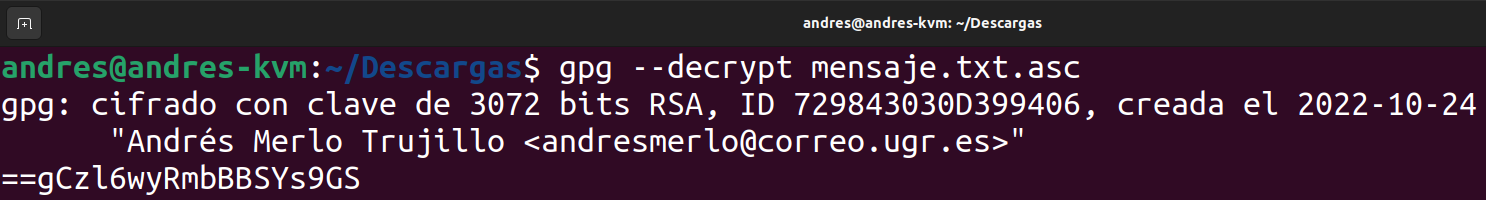
\includegraphics[width=\textwidth]{imagenes/Portatil/Captura desde 2022-10-24 12-18-40.png}
    \caption{Desencriptado del mensaje con mi clave privada.}
\end{figure}

Como se puede ver, también ha ``encriptado'' el mensaje del interior, se puede observar que al principio tiene dos símbolos ``='', señal de que ha usado base64 y le ha dado la vuelta. Para desencriptarlo del todo, es necesario usar la orden \verb|echo "msg"| $\vert$ \verb|rev| $\vert$ \verb|base64 -d|:

\begin{figure}[H]
    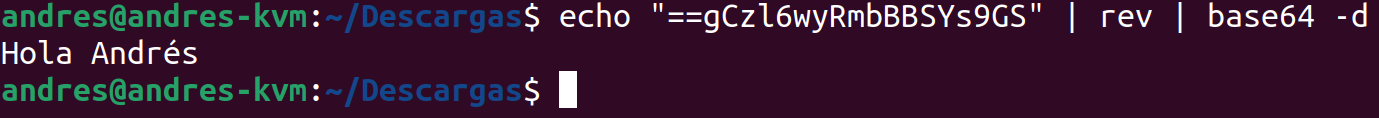
\includegraphics[width=\textwidth]{imagenes/Portatil/base64.png}
    \caption{Desencriptado del base64 realizado.}
\end{figure}

Y finalmente se puede leer el mensaje sin problema alguno.

\newpage

\phantomsection
\addcontentsline{toc}{section}{Ejercicio 2}
\section*{Ejercicio 2}

\textbf{Enunciado: }``Utiliza la herramienta \texttt{openssl} para cifrar y descifrar un archivo con un algoritmo y clave de tu elección.''

\bigskip

Voy a cifrar el siguiente archivo:

%Captura desde 2022-10-19 17-33-08
\begin{figure}[H]
    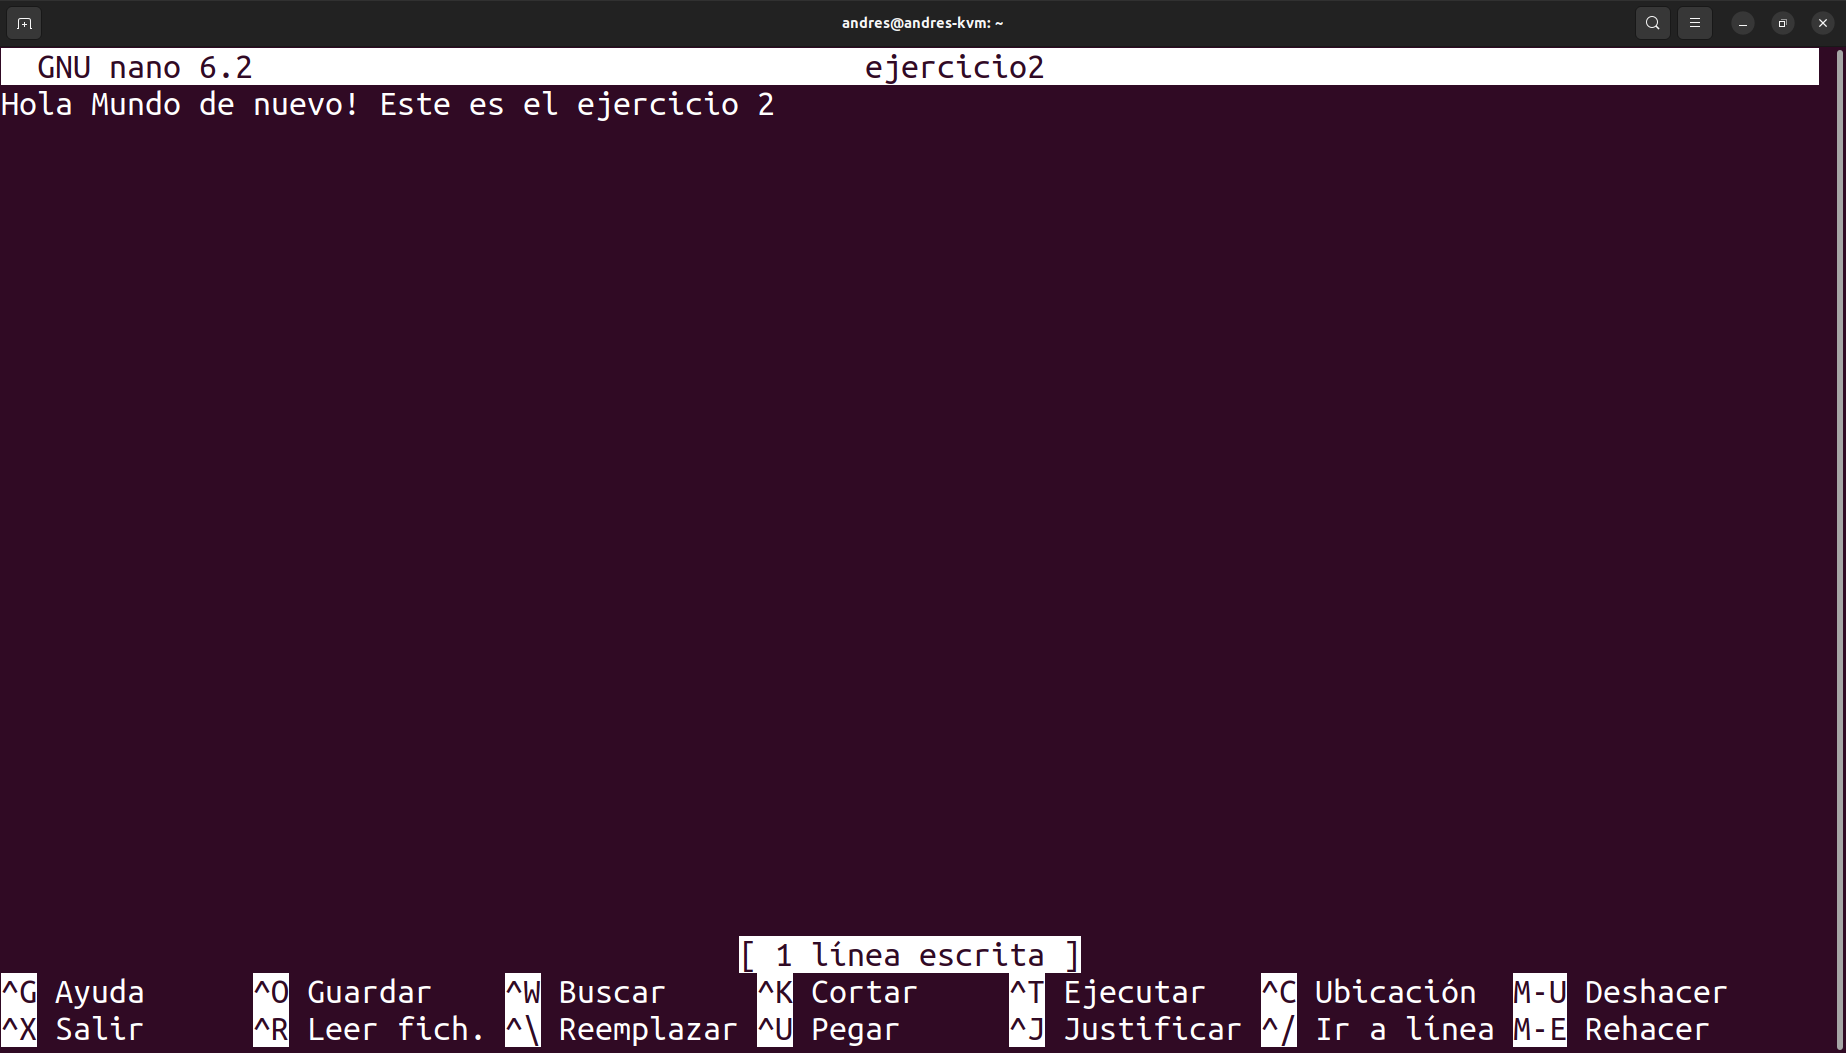
\includegraphics[width=\textwidth]{imagenes/Captura desde 2022-10-19 17-33-08.png}
    \caption{Contenido del archivo a cifrar.}
\end{figure}

El algoritmo de cifrado que voy a usar es ``desx'' y voy a usar 1234 iteraciones y con la contraseña ``qwerty''. Por tanto, para realizar esto, es necesario usar la orden 

\verb|openssl enc -des3 -iter 1234 -in ejercicio2 -out cifrado|

%Captura desde 2022-10-19 17-44-41
\begin{figure}[H]
    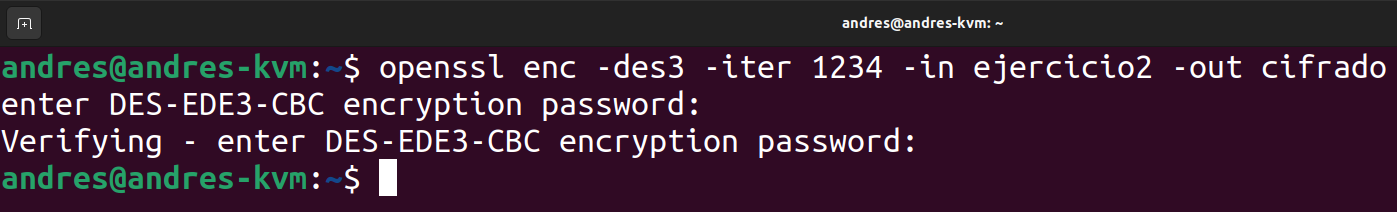
\includegraphics[width=\textwidth]{imagenes/Captura desde 2022-10-19 17-44-41.png}
    \caption{Encriptación del archivo.}
\end{figure}

Como se puede observar, pide la contraseña para encriptar, que es ``qwerty'' como he dicho antes. 

\bigskip

Ahora al mostrar el contenido del archivo cifrado, se ve que no es entendible:

%Captura desde 2022-10-19 17-44-49
\begin{figure}[H]
    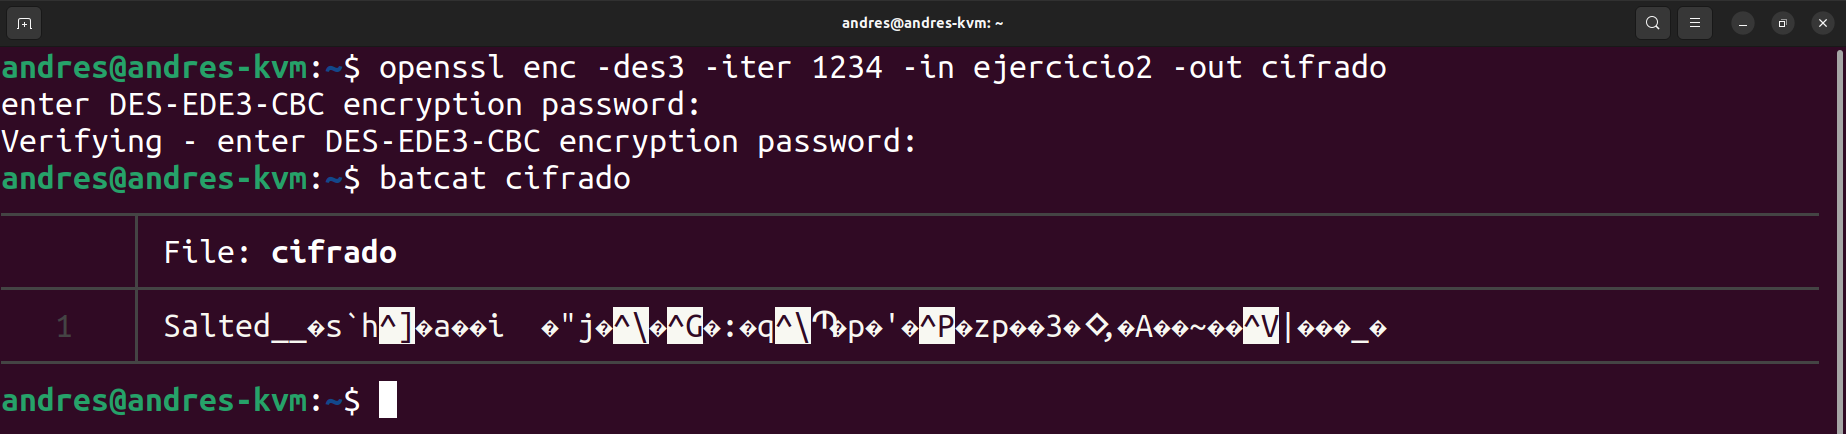
\includegraphics[width=\textwidth]{imagenes/Captura desde 2022-10-19 17-44-49.png}
    \caption{Salida del archivo cifrado.}
\end{figure}


Y ahora para descifrarlo, simplemente hace falta saber la contraseña, el algoritmo de cifrado y el número de iteraciones. 

\bigskip

Todo esto se debe poner en el comando: \verb|openssl enc -des3 -iter 1234 -d -in cifrado|

%Captura desde 2022-10-19 17-54-02
\begin{figure}[H]
    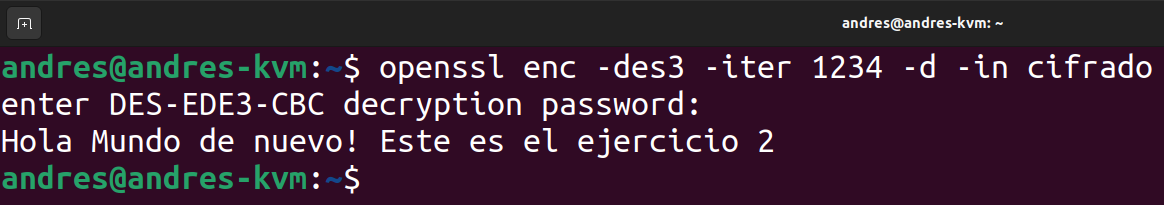
\includegraphics[width=\textwidth]{imagenes/Captura desde 2022-10-19 17-54-02.png}
    \caption{Desencriptado del mensaje cifrado.}
\end{figure}

\end{document}

%\begin{figure}[H]
%    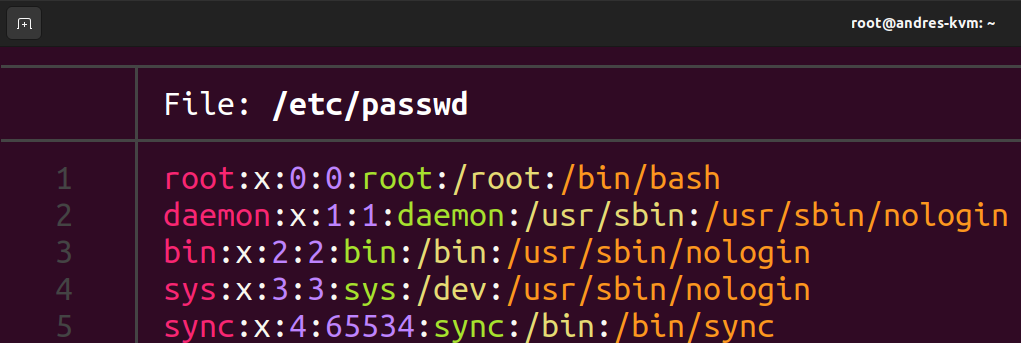
\includegraphics[width=\textwidth]{imagenes/passwdfile.png}
%    \caption{Ejemplo de entradas en el archivo.}
%\end{figure}